 \chapter{Diseño y selección de componentes}

 \graphicspath{{Chapter4/Figuras/}{Chapter4/Figs/PDF/}{Chapter4/Figs/}}

El sistema a diseñar se divide en dos partes, El dispositivo físico que se tendrá en cada auto y el procesamiento que se llevará a cabo en la nube. Se empezará diseñando el dispositivo físico para luego integrarlo con el procesamiento en la nube.

\section{Dispositivo físico}
El dispositivo físico seguirá el diagrama de bloques mostrado en Fig.~\ref{fig:bloques}. Se procederá a seleccionar cada componente del mismo.

\begin{figure}[htbp!]
\centering
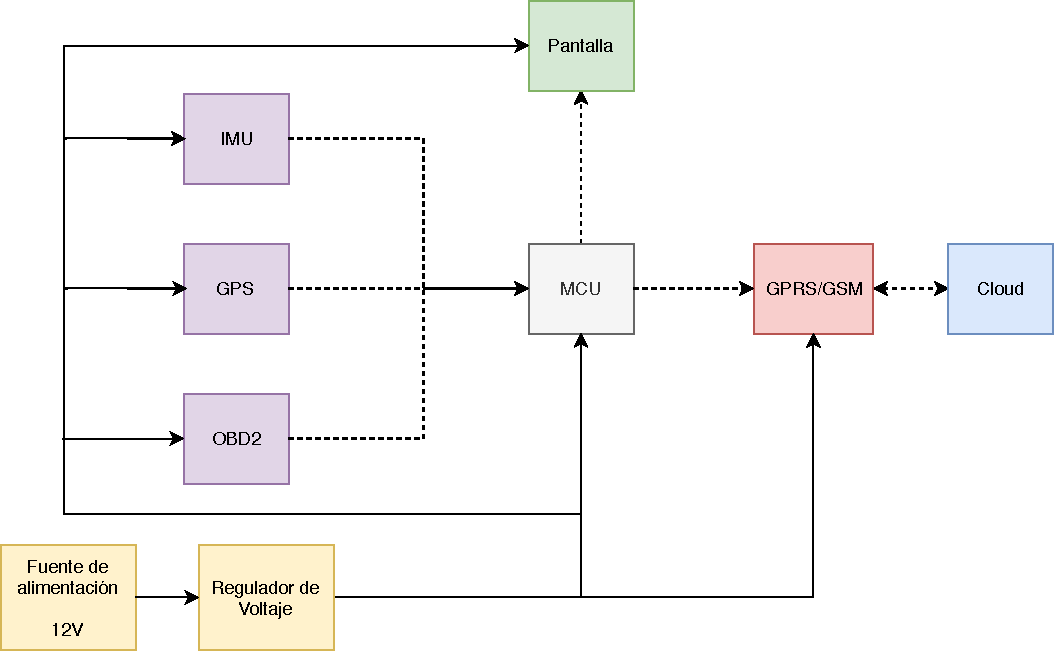
\includegraphics[width=0.9\textwidth]{Bloques.pdf}
\caption{Diagrama de bloques del dispositivo físico.}
\label{fig:bloques}
\end{figure}

\subsection{Selección del IMU}
Este dispositivo cuenta con un acelerómetro, un giroscopio y un magnetómetro. Los datos registrados por estos sensores se pueden combinar para obtener el perfil de velocidad y aceleración, tanto longitudinal como lateral, del vehículo y estos perfiles aportan mucha información acerca del estilo de conducción del usuario.

Para seleccionar este componente empecemos por determinar las características que este debe poseer. En primer lugar el rango de medición debe ser el adecuado. En las investigaciones citadas  \cite{6957822}, \cite{constantinescu}, \cite{6083078},  \cite{Va-2013} La aceleración de los vehículos se suele encontrar dentro del rango de \SI{\pm7}{m/s^2}. Los rangos de medición de los acelerómetros se suelen expresar en \SI{}{g}, así que se necesita un acelerómetro que pueda medir en un rango de por lo menos \SI{\pm0.7}{g}

Realizando el mismo análisis para el giroscopio, en \cite{6083078} y \cite{6629603} se tiene que el rango mínimo de medición es de \SI{\pm57}{rad/s}

El sensor que se eligió debido a que cumple con las características mencionadas anteriormente es el \textbf{ICM-20648} (Fig.~\ref{fig:IMU}) producido por TDK InvenSense. En las Tablas \ref{diag:IMU1} y \ref{diag:IMU2} se muestran sus principales características.

\bgroup
\def\arraystretch{1.5}%  1 is the default, change whatever you need
\begin{table}[htbp!]
\centering
\caption[Sensibilidad y Rango del ICM-20648]{Sensibilidad y Rango del ICM-20648 \cite{ICM20648}.}
\begin{tabular}{@{}P{3cm}P{3cm}P{3cm}P{3cm}@{}}
\toprule
Rango del Giroscopio (\si{\degree/sec}) & Sensibilidad del Giroscopio (\si{LSB/\degree/sec}) & Rango del Acelerómetro     (\si{g}) & Sensibilidad del Acelerómetro (\si{LSB/g}) \\ \midrule
\num{\pm 250} & 131 & \num{\pm 2} & 16384 \\
\num{\pm 500} & 65.5 & \num{\pm 4} & 8192 \\
\num{\pm 1000} & 32.8 & \num{\pm 8} & 4096 \\
\num{\pm 2000} & 16.4 & \num{\pm 16} & 2048 \\ \bottomrule
\end{tabular}
\label{diag:IMU1}
\end{table}

\begin{table}[htbp!]
\centering
\caption[Condiciones de Operación del ICM-20648]{Condiciones de Operación del ICM-20648 \cite{ICM20648}.}
\begin{tabular}{@{}P{3.2cm}P{3.2cm}P{3.2cm}P{3.2cm}@{}}
\toprule
Salida Digital & Voltaje de Alimentación & Corriente de Operación & Temperatura de Operación \\ \midrule
I\textsuperscript{2}C o SPI & \SI{1.71}{V} - \SI{3.6}{V} & \SI{3.2}{mA} & \SI{-40}{\celsius} hasta \SI{85}{\celsius} \\ \bottomrule
\end{tabular}
\label{diag:IMU2}
\end{table}

\egroup

\begin{figure}[htbp!]
\centering
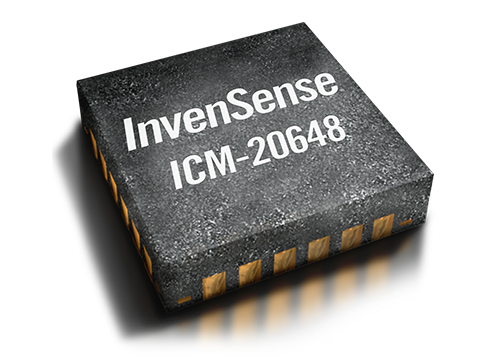
\includegraphics[width=0.4\textwidth]{ICM-20648.png}
\caption{ICM-20648, IMU de 6 grados de libertad.}
\label{fig:IMU}
\end{figure}

A partir de las características señaladas se realiza el esquemático (Fig.~\ref{fig:IMU_esquem}) de las conexiones necesarias para poder alimentar al módulo y para que este pueda comunicarse con el microcontrolador. Se establece el voltaje de alimentación y el voltaje lógico a \SI{3.3}{V}. En \cite{ICM20648} se recomiendan los valores de los capacitores y se conectan los pines necesarios para poder implementar el protocolo de comunicación I\textsuperscript{2}C. El pin 9 se conecta a GND para establecer la dirección I\textsuperscript{2}C a b1101000.

\begin{figure}[htbp!]
\centering
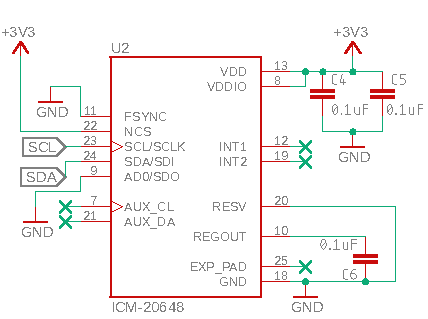
\includegraphics[width=0.9\textwidth]{IMU_esquem.pdf}
\caption{Esquemático del módulo ICM-20648.}
\label{fig:IMU_esquem}
\end{figure}

\subsection{Selección del módulo GPS}
Este módulo se encargará de detectar la posición exacta del vehículo en coordenadas. Para hacer esto se puede recurrir a distintos servicios del Sistema mundial de navegación por satélite (GNSS). Actualmente se encuentran dos operativos completamente: GPS y GLONASS. Es primero es el servicio hecho por Estados Unidos y el segundo es el realizado por Rusia. Es importante considerar la capacidad de los diferentes módulos para poder acceder a estos dos servicios.

Las características que debe tener el módulo de GPS son las siguientes:
\begin{itemize}
    \itemsep0em
    \item Bajo consumo.
    \item Poder acceder tanto a GPS como a GLONASS.
    \item Por lo menos una frecuencia de muestreo de \SI{1}{Hz}.
\end{itemize}

El modulo de GPS que cumple con estas características es el \textbf{NEO-M8N} de Ublox (Fig.~\ref{fig:GPS}). En la Tabla~\ref{diag:GPS} se resumen sus principales características.
\begin{figure}[hbtp!]
\centering
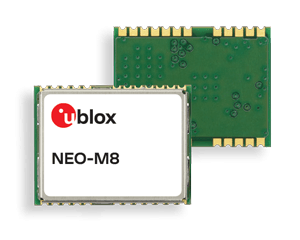
\includegraphics[width=0.5\textwidth]{NEO-M8.png}
\caption[NEO-M8N, módulo GPS]{NEO-M8N, módulo GPS \cite{GPS}.}
\label{fig:GPS}
\end{figure}

\bgroup
\def\arraystretch{1.5}%  1 is the default, change whatever you need
\begin{table}[htbp!]
\centering
\caption[Características del NEO-M8N]{Características del NEO-M8N \cite{GPS}.}
\begin{tabular}{@{}ll@{}}
\toprule
Características & Valor \\ \midrule
GNSS & GPS, GLONASS, GALIEO y BeiDou \\
Precisión & \SI{2.5}{m} \\
Frecuencia máxima & \SI{5}{Hz} \\
Protocolos de Comunicación & UART, I\textsuperscript{2}C, SPI \\
Voltaje de operación & \SI{2.7}{V} - \SI{3.6}{V} \\
Corriente de operación & \SI{32}{mA} \\
Corriente máxima & \SI{67}{mA} \\
Temperatura de Operación & \SI{-40}{\celsius} hasta \SI{85}{\celsius} \\\bottomrule
\end{tabular}
\label{diag:GPS}
\end{table}
\egroup

A partir de los parámetros mencionados se realiza el esquemático (Fig.~\ref{fig:GPS_esquem}) de las conexiones necesarias para alimentar al módulo e implementar la comunicación con el microcontrolador. En este caso se alimenta al módulo con \SI{3.3}{V} y se implementa comunicación serial con el microcontrolador. Además se tiene un conector SMA para poder conectar una antena externa y también se cuenta con una batería de \SI{3}{V} con una capacidad de \SI{5}{mAh} según \cite{MS621FE}.

Esta batería se encargará de mantener activo al módulo GPS en modo de bajo consumo durante la noche cuando la fuente de voltaje principal este desconectada. Esto se quiere hacer debido a que el GPS encontrará la posición de una forma más rápida si se mantiene activo. En cambio, cuando se apaga y se vuelve a encender se le llama "encendido en frío" y toma más tiempo.

\begin{figure}[htbp!]
\centering
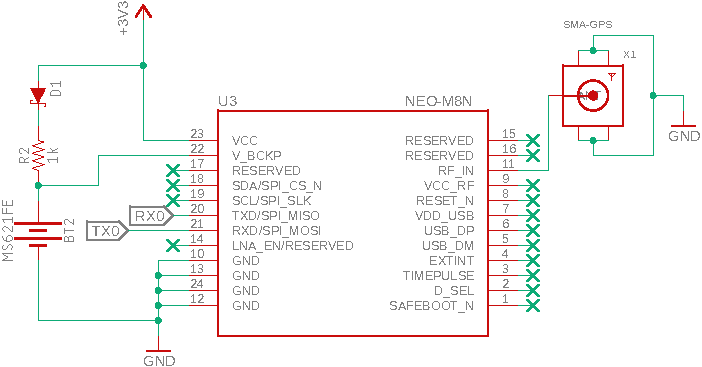
\includegraphics[width=\textwidth]{GPS_esquem.pdf}
\caption{Esquemático del módulo NEO-M8N.}
\label{fig:GPS_esquem}
\end{figure}

\subsection{Selección del módulo GPRS/GSM}
El módulo GPRS/GSM es capaz de conectarse a las red 2G. Esta red es la que tiene mayor cobertura en el Perú (Fig.~\ref{fig:Cobertura}) ya que es la más antigua. Esta red puede alcanzar hasta una velocidad de \SI{114}{kbps} y es la de menor consumo energético, comparada con 3G y 4G. Usando este módulo se enviarán los datos recopilados por el sistema a través de Internet y se asegurará su conexión en todo momento.

\begin{figure}[hbtp!]
\centering
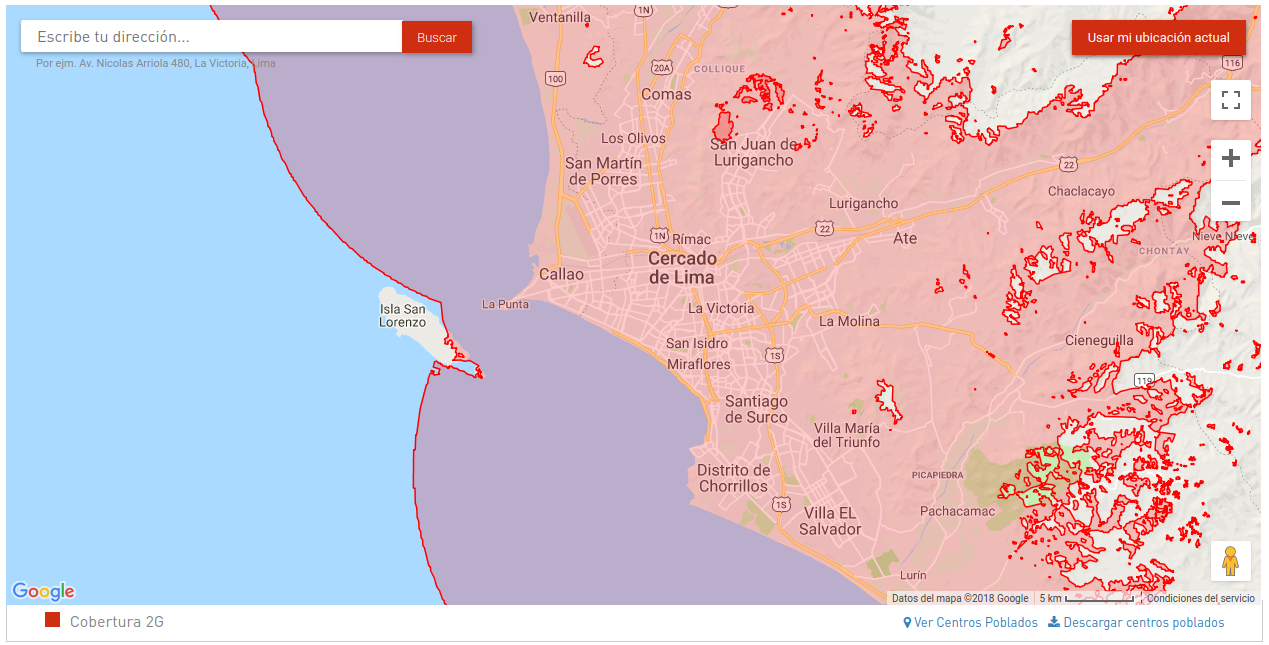
\includegraphics[width=\textwidth]{Cobertura_2G.png}
\caption[Cobertura de la red 2G de Claro]{Cobertura de la red 2G de Claro \cite{Cobertura_claro}.}
\label{fig:Cobertura}
\end{figure}

Una opción muy popular es el módulo \textbf{SIM 800L} (Fig.~\ref{fig:SIM}) que debido a sus características, expuestas en la Tabla~\ref{diag:SIM}, su disponibilidad y su bajo precio lo hacen adecuado para ser usado en este sistema.

\begin{figure}[hbtp!]
\centering
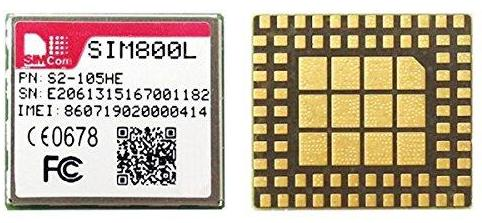
\includegraphics[width=0.6\textwidth]{SIM800L.jpg}
\caption[SIM 800L, módulo GPRS/GSM]{SIM 800L, módulo GPRS/GSM \cite{SIM800L}.}
\label{fig:SIM}
\end{figure}

\bgroup
\def\arraystretch{1.5}%  1 is the default, change whatever you need
\begin{table}[htbp!]
\centering
\caption[Características del SIM 800L]{Características del SIM 800L \cite{SIM800L}.}
\begin{tabular}{@{}p{5.4cm}p{8cm}@{}}
\toprule
Características & Valor \\ \midrule
Voltaje de operación & \SI{3.4}{V} -  \SI{4.4}{V} \\
Corriente promedio en Reposo & \SI{18.7}{mA} \\
Corriente promedio durante \mbox{transmisión} & \SI{453.57}{mA} \\
Corriente máxima & \SI{2}{A} (Solo durante ráfaga de transmisión) \\
Temperatura de operación & \SI{-40}{\celsius} hasta \SI{85}{\celsius} \\
Velocidad de transmisión & máx. \SI{85.6}{kbps} \\
Bandas de frecuancia & Quad-band: GSM 850, EGSM 900, DCS 1800, PCS 1900 \\ \bottomrule
\end{tabular}
\label{diag:SIM}
\end{table}
\egroup

\begin{figure}[htbp!]
\centering
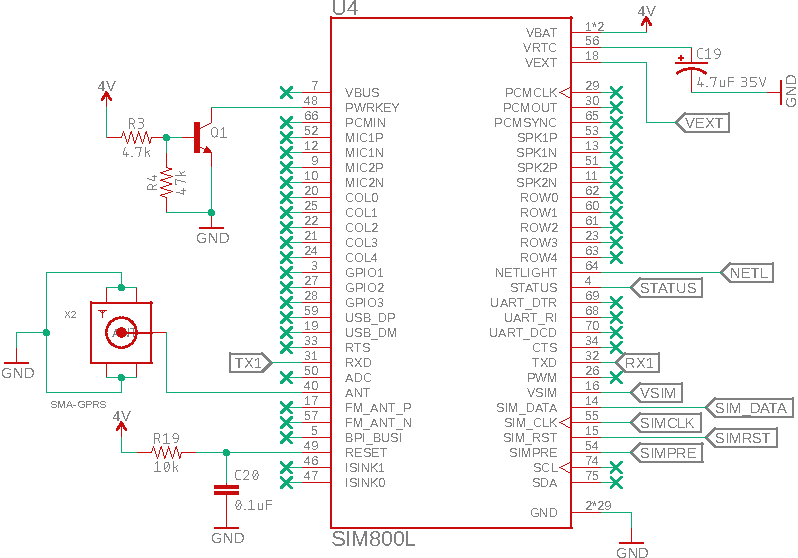
\includegraphics[width=\textwidth]{GSM_esquem.pdf}
\caption{Esquemático del módulo SIM800L.}
\label{fig:GSM_esquem}
\end{figure}

A partir de los parámetros mencionados en la Tabla~\ref{diag:SIM} se realiza el esquemático (Fig.~\ref{fig:GSM_esquem}) de las conexiones necesarias para alimentar al módulo e implementar la comunicación con el microcontrolador.



En este caso el módulo es alimentado con \SI{4}{V} y se usará comunicación serial. Los capacitores elegidos son recomendaciones de \cite{SIM800L} al igual que el transistor que cumplirá la función de encender y apagar correctamente el módulo.


Además se necesita de un módulo que lea una tarjeta SIM. En la Fig.~\ref{fig:GSM_SIM_esquem} se muestra el esquemático de este módulo, el lector de tarjetas SIM (SIM8055). La conexión mostrada es recomendada en \cite{SIM800L}.

\begin{figure}[htbp!]
\centering
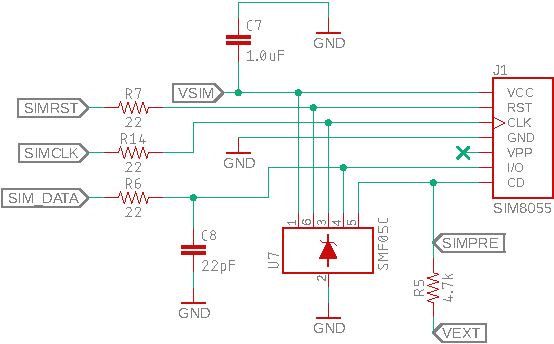
\includegraphics[width=\textwidth]{GSM_SIM_esquem.pdf}
\caption{Esquemático del módulo SIM8055.}
\label{fig:GSM_SIM_esquem}
\end{figure}

Por último, se tiene en la Fig.~\ref{fig:GSM_LED_esquem} el esquemático de la conexión de dos LEDs que servirán para indicar el estado de la conexión a internet del módulo y también si este se encuentra encendido o no. Se usará un conector para cablear los LEDs ya que estos no se encontrarán soldados a la PCB porque se necesitan en una posición específica del case del dispositivo.

\begin{figure}[htbp!]
\centering
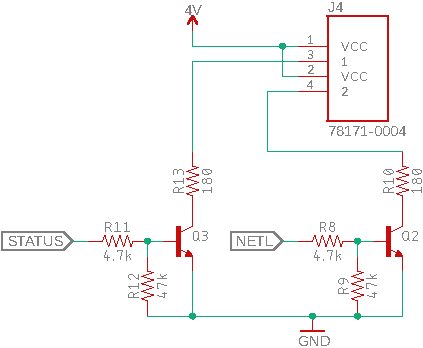
\includegraphics[width=0.7\textwidth]{GSM_LED_esquem.pdf}
\caption{Esquemático las los indicadores LED.}
\label{fig:GSM_LED_esquem}
\end{figure}

\subsection{Selección de la Pantalla}
La pantalla cumplirá el rol de mostrar la clasificación del estilo de conducción del usuario. Para poder transmitir la información sin generar distracciones se usarán símbolos y colores para representar los estilos de conducción.

Además se necesita que la pantalla se pueda observar bien tanto a la luz del día, por lo que su ángulo de visibilidad y su brillo serán factores importantes también.

Por último, el tamaño de la pantalla debe permitir la identificación del símbolo por parte del conductor. Basados en estos parámetros se puede elegir entre usar 3 tecnologías muy populares: LCD, OLED e IPS LCD.

Las pantallas LCD pueden alcanzar una densidad de imagen más alta que las OLED. Sin embargo, las OLED tienen un mejor ángulo de visión y un menor consumo. Por otro lado, las IPS LCD tienen también un muy buen ángulo de visión y buena densidad de imagen.

En la Tabla.~\ref{diag:Display} se pueden ver 3 alternativas para la pantalla. De estas se escoge la pantalla IPS LCD (Fig.~\ref{fig:Display}), ya que tiene buen ángulo de visibilidad, tamaño y resolución.

\bgroup
\def\arraystretch{1.5}%  1 is the default, change whatever you need
\begin{table}[htbp!]
\centering
\caption{Alternativas de pantallas}
\begin{tabular}{@{}p{1.6cm}lllP{3cm}lc@{}}
\toprule
Nr. \mbox{Producto} & Tecnología & Controlador & Tamaño & Voltaje de Operación & Precio & Resolución\\ \midrule
1431 & OLED & SSD1351 & \SI{1.5}{in} & \SI{3.3}{V} o \SI{5}{V} & \textdollar \num{39.95} & 128x128\\
2088 & LCD & ST7735R & \SI{1.44}{in} & \SI{3.3}{V} o \SI{5}{V} & \textdollar \num{14.95} & 128x128\\
3787 & IPS LCD & ST7789 & \SI{1.54}{in} & \SI{3.3}{V} o \SI{5}{V} & \textdollar \num{19.95} & 240x240\\ \bottomrule
\end{tabular}
\label{diag:Display}
\end{table}
\egroup


\begin{figure}[hbtp!]
\centering
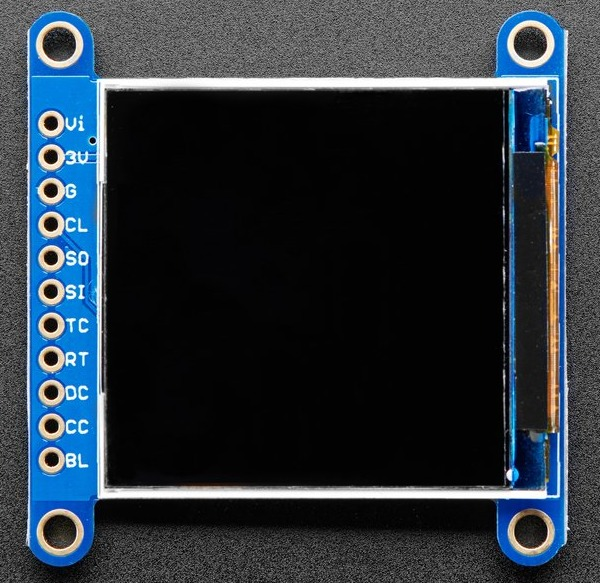
\includegraphics[width=0.8\textwidth]{IPS_LCD.jpg}
\caption[Adafruit 1.54" 240x240 Wide Angle TFT LCD Display - ST7789]{Adafruit 1.54" 240x240 Wide Angle TFT LCD Display - ST7789 \cite{IPS_LCD}.}
\label{fig:Display}
\end{figure}

La pantalla se colocará fuera del case donde estará el PCB por lo que se usarán borneras para conectar los pines necesarios al microcontrolador, como indica la Fig.~\ref{fig:DISPLAY_esquem}. Se usa el protocolo SPI para comunicarse con el microcontrolador y se alimenta a la pantalla con \SI{3.3}{V}. Además se usan solo 8 pines ya que estos son los únicos necesarios para controlar la pantalla.

\begin{figure}[htbp!]
\centering
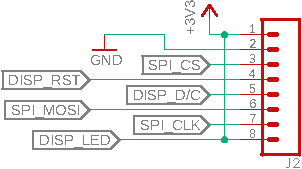
\includegraphics[width=0.6\textwidth]{DISPLAY_esquem.pdf}
\caption{Esquemático bornera para conectar la pantalla.}
\label{fig:DISPLAY_esquem}
\end{figure}

\subsection{Selección del módulo OBD2}
Este módulo se encargará de acceder a todos los parámetros internos del auto conectándose directamente a las ECU \textit{(Electronic Control Units)} del motor. Para poder leer estos parámetros diversas marcas de autos usan distintos protocolos de comunicación. En la Tabla~\ref{diag:OBD} Se muestran distintos protocolos y en cada columna circuitos integrados ELMXXX que se usan para comunicarse con el puerto OBD2.

\bgroup
\def\arraystretch{1.5}%  1 is the default, change whatever you need
\begin{table}[htbp!]
\centering
\caption[Protocolos y Circuitos integrados]{Protocolos y Circuitos integrados \cite{OBD}.}
\begin{tabular}{|l|P{1.5cm}|P{1.5cm}|P{1.5cm}|P{1.5cm}|P{1.8cm}|}
\hline
 &  ELM323 & ELM325 & ELM327  & ELM329 & ELM329L \\ \hline
SAE J1850-PWM   &  &  & \si{\surd}  &  &  \\ \hline
SAE J1850-VPW   &  &  & \si{\surd}  &  &  \\ \hline
ISO 9141-2   & \si{\surd} &  & \si{\surd}  &  &  \\ \hline
ISO 14230-4 (slow)     & \si{\surd} &  & \si{\surd}  &  &  \\ \hline
ISO 14230-4 (fast)     & \si{\surd} &  & \si{\surd} &  \si{\surd} & \si{\surd} \\ \hline
ISO 15765-4 (CAN)     &  &  & \si{\surd} & \si{\surd} &  \si{\surd} \\ \hline
SAE J1939 (250kbps)     &  &  & \si{\surd} & \si{\surd} &  \si{\surd} \\ \hline
SAE J1939 (500kbps)     &  &  & \si{\surd} & \si{\surd} & \si{\surd} \\ \hline
SAE J1708 (J1587)     &  & \si{\surd} &  &    &  \\ \hline
SAE J1708 (J1922)     &  & \si{\surd} &  &    &  \\ \hline
\end{tabular}
\label{diag:OBD}
\end{table}
\egroup

Para maximizar la compatibilidad con vehículos se escoge el modulo \textbf{ELM327}. Este IC convierte los protocolos mencionados a comunicación serial y puede transmitir los datos a través de un cable, WiFi o Bluetooth. Para esta aplicación se escoge la versión que usa Bluetooth (Fig.~\ref{fig:OBD}) ya que el conector se encontrará a menos de \SI{2}{m} del conector, permitiéndole usar esta tecnología que consume menos energía que el WiFi y es inalámbrica también.

\begin{figure}[hbtp!]
\centering
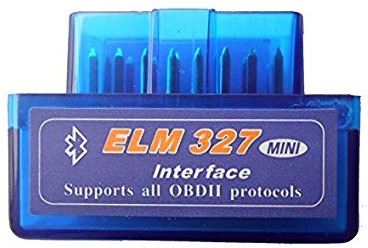
\includegraphics[width=0.35\textwidth]{OBD.jpg}
\caption[ELM327 - OBD2 interface]{ELM327 - OBD2 interface \cite{OBD}.}
\label{fig:OBD}
\end{figure}

\subsection{Selección del Microcontrolador}
El microcontrolador a seleccionar necesita poder comunicarse con todos los módulos anteriores, poder manejar protocolos como MQTT y CoAP y además realizar procesamiento básico de fusión de sensores (mezclar los datos obtenidos del IMU y del GPS). Se ha escogido para este sistema al ESP-WROOM-32 (Fig.~\ref{fig:esp-wroom32})

Este microcontrolador cuenta con el diagrama de bloques expuesto en la Fig.~\ref{fig:Bloques_esp32} y como se puede apreciar, cuenta con I\textsuperscript{2}C para comunicarse con el IMU, UART para comunicarse con el módulo GPS y el módulo GPRS/GSM, SPI para controlar la pantalla y Bluetooth para comunicarse con el módulo OBD2. Además presenta la suficiente potencia para realizar las tareas anteriormente descritas. Un resumen de sus características se encuentra en la Tabla~\ref{diag:ESP32}.

\begin{figure}[hbtp!]
\centering
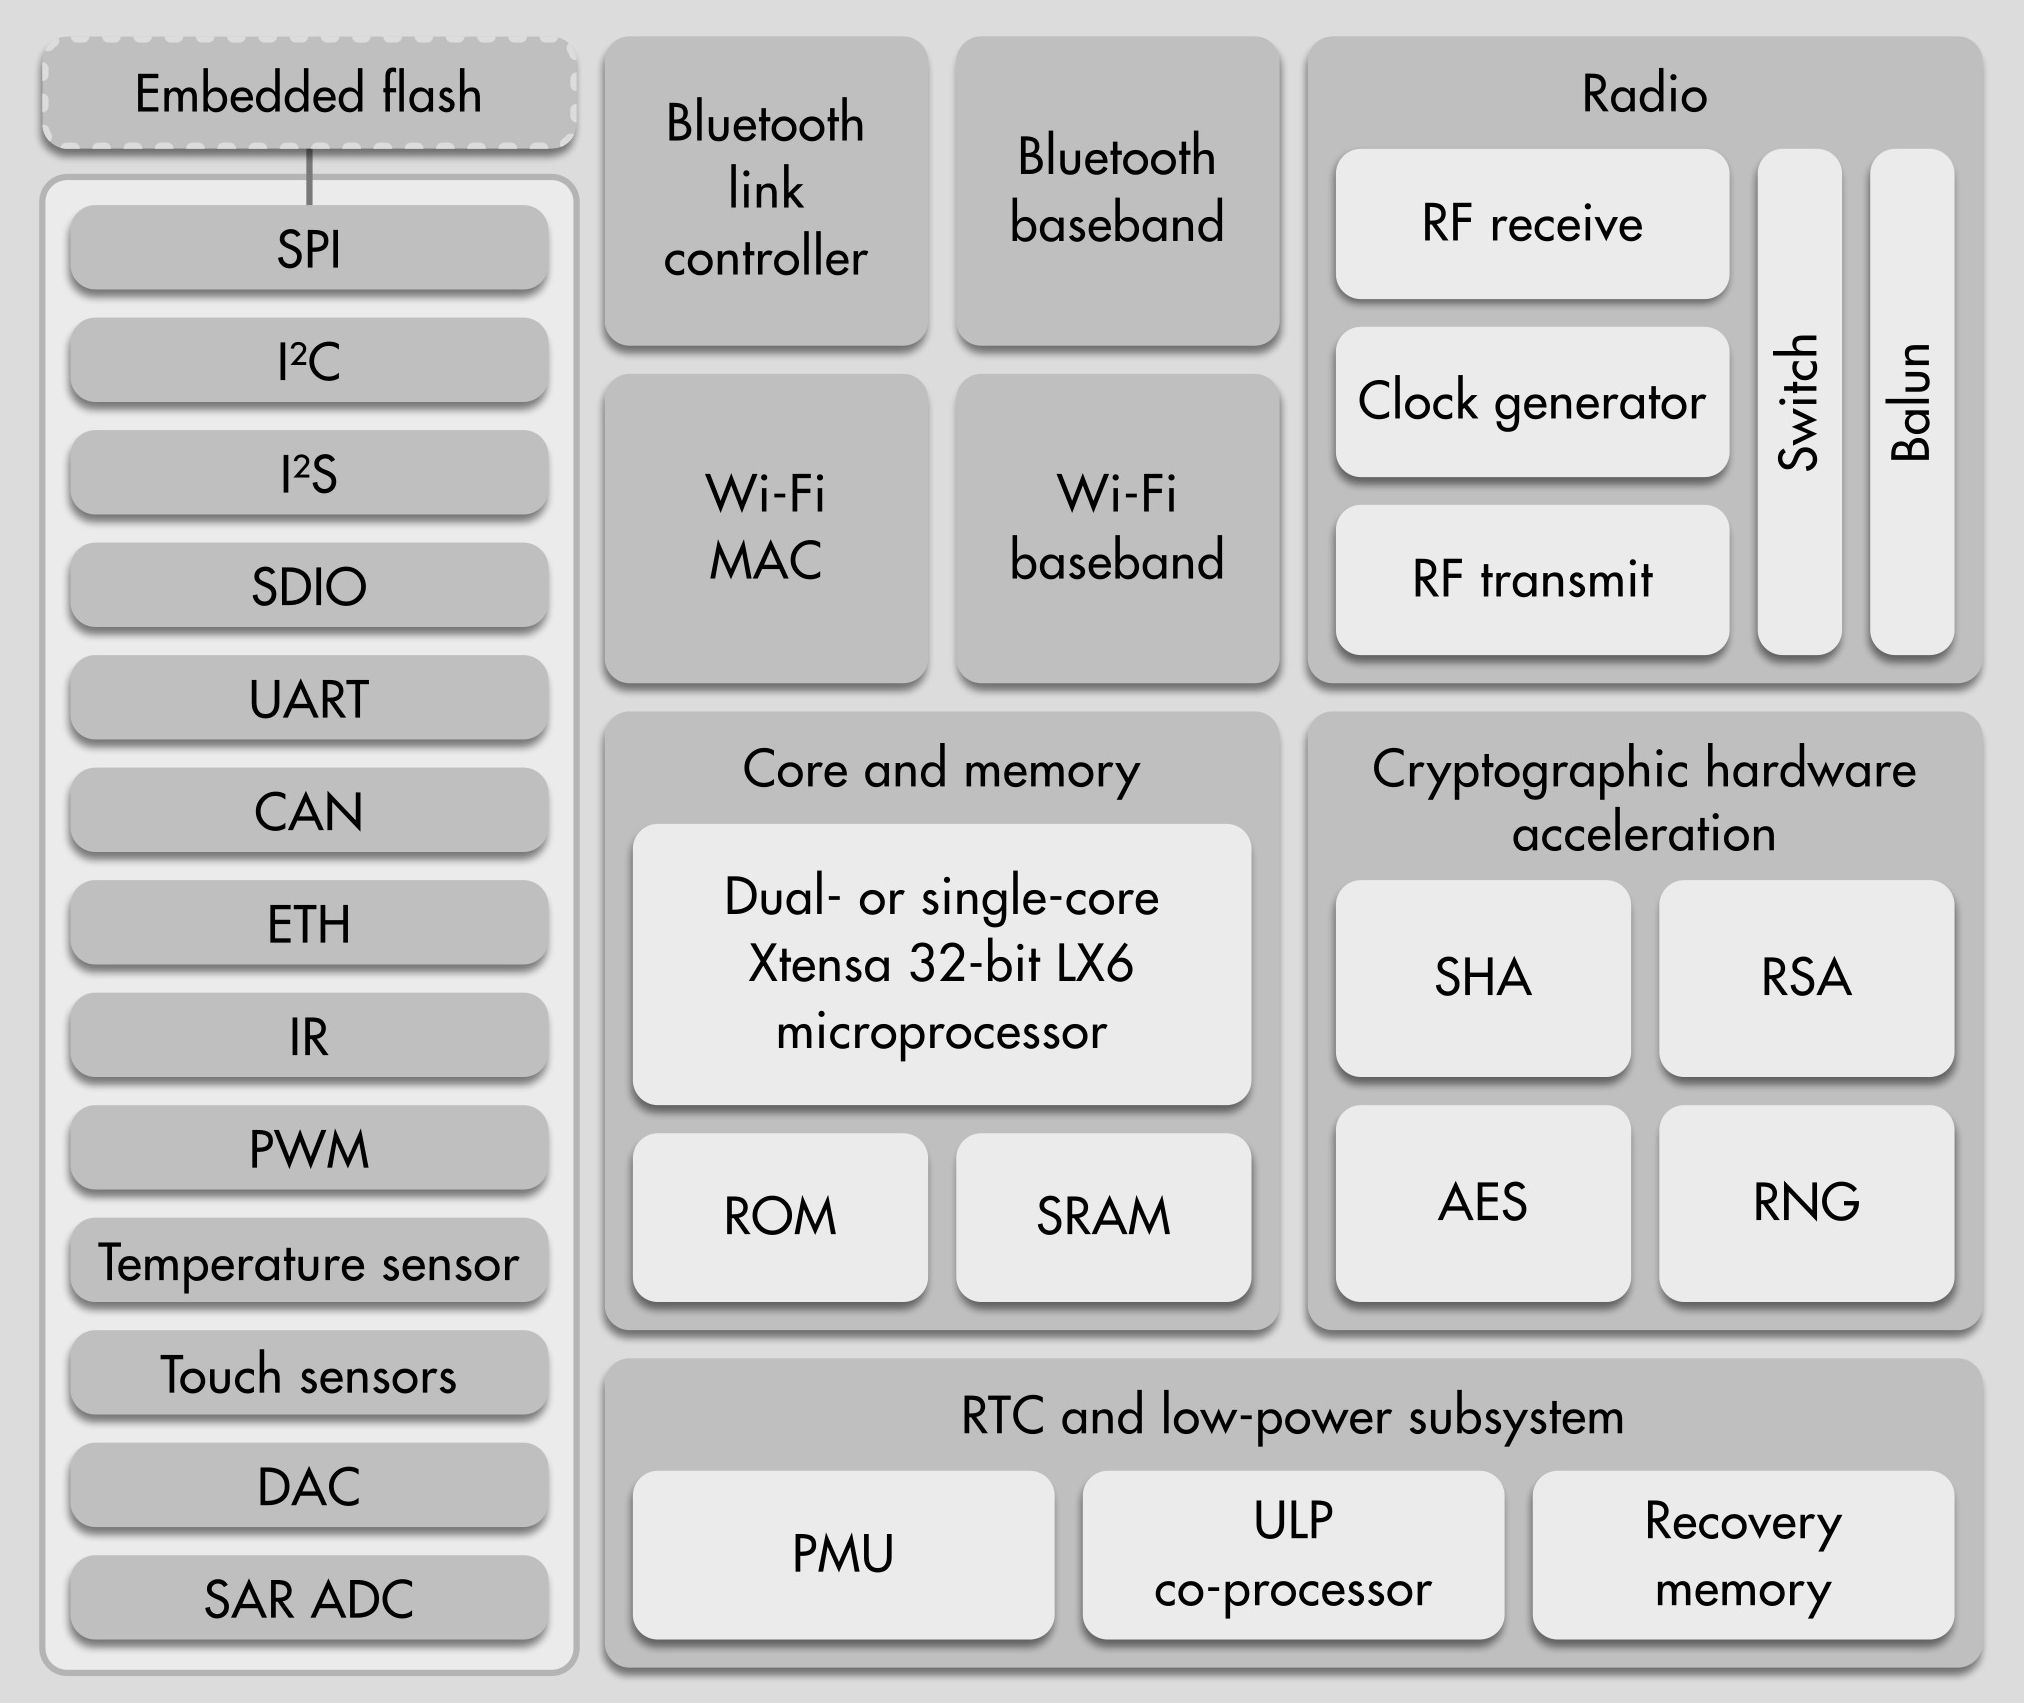
\includegraphics[width=0.9\textwidth]{ESP32_Function_Block_Diagram.jpg}
\caption{Diagrama de Bloques del ESP32  \cite{Esp32}.}
\label{fig:Bloques_esp32}
\end{figure}


\begin{figure}[hbtp!]
\centering
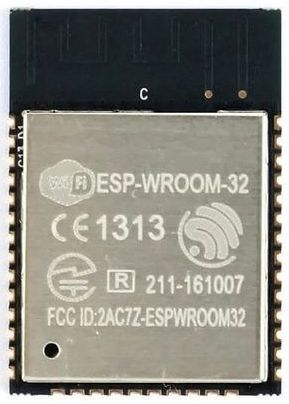
\includegraphics[width=0.3\textwidth]{esp32.jpg}
\caption{ESP-WROOM-32 \cite{ESP32_page}.}
\label{fig:esp-wroom32}
\end{figure}

\bgroup
\def\arraystretch{1.5}%  1 is the default, change whatever you need
\begin{table}[htbp!]
\centering
\caption[Características del ESP-WROOM-32]{Características del ESP-WROOM-32 \cite{Esp32_Hardware}.}
\begin{tabular}{@{}lp{9cm}@{}}
\toprule
Características & Valor \\ \midrule
Voltaje de Operación & \SI{2.7}{V} - \SI{3.6}{V} \\
Corriente máxima & \SI{500}{mA} \\
Corriente de operación & \SI{80}{mA} \\
Corriente en sleep mode & \SI{5}{\uA} \\
Frecuencia del CPU & \SI{240}{MHz} \\
Temperatura de operación & \SI{-40}{\celsius} hasta \SI{85}{\celsius} \\
Interfaces & SD card, UART, SPI, SDIO, I\textsuperscript{2}C, LED PWM, Motor PWM, I 2 S,IR, contador de pulsos, GPIO, sensor táctil capacitivo, ADC, DAC \\
Connectividad & WiFi (802.11 b/g/n (802.11n up to 150 Mbps) Bluetooth (Bluetooth v4.2 BR/EDR y BLE)\\\bottomrule
\end{tabular}
\label{diag:ESP32}
\end{table}
\egroup

En la Fig.~\ref{fig:ESP_esquem} se muestra el esquemático del microcontrolador y su alimentación. En \cite{Esp32_Hardware} se recomienda usar los capacitores que se encuentran conectados al microcontrolador y se muestran también todas las conexiones de los módulos anteriores; 1 conexión I\textsuperscript{2}C, 2 conexiones seriales y 1 conexión SPI.

\begin{figure}[hbtp!]
\centering
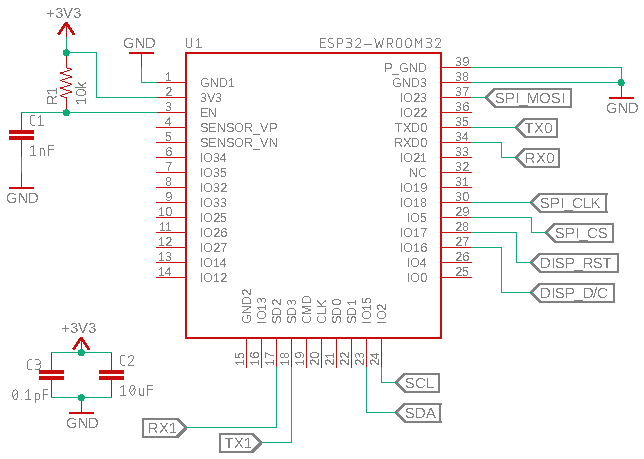
\includegraphics[width=\textwidth]{ESP32_esquem.pdf}
\caption{Esquemático de la implementación del ESP-WROOM-32.}
\label{fig:ESP_esquem}
\end{figure}

\subsection{Diseño de la etapa de alimentación}
Una vez escogidos los componentes a usar en las secciones anteriores, se calculará el consumo total de los componentes para poder diseñar la etapa de alimentación del sistema. En la Tabla~\ref{diag:consumo} se encuentra un resumen de cada dispositivo con su voltaje de operación y su corriente máxima de consumo.

\bgroup
\def\arraystretch{1.5}%  1 is the default, change whatever you need
\begin{table}[htbp!]
\centering
\caption[Consumo de los componentes del sistema]{Consumo de los componentes del sistema.}
\begin{tabular}{@{}lp{2cm}p{2cm}p{2cm}@{}}
\toprule
Dispositivo & Voltaje de Operación & Corriente máxima & Potencia máxima\\ \midrule
IMU (ICM-20648) & \SI{3.3}{V} & \SI{3.2}{\mA} & \SI{10.56}{\mW} \\
Módulo GPS (NEO-M8N) & \SI{3.3}{V} & \SI{67}{mA} & \SI{221,1}{\mW}\\
Módulo GPRS/GSM (SIM800L) & \SI{4}{V} & \SI{2000}{mA} & \SI{8000}{\mW}\\
Pantalla IPS LCD & \SI{3.3}{V} & \SI{50}{mA} & \SI{165}{\mW}\\
OBD2 (ELM237) & \SI{5}{V} & \SI{12}{mA} & \SI{60}{\mW}\\
ESP-WROOM-32 & \SI{3.3}{V} & \SI{500}{mA} & \SI{1650}{\mW}\\ \bottomrule
\end{tabular}
\label{diag:consumo}
\end{table}
\egroup

Sin embargo, El módulo OBD2 (ELM237) no estará conectado junto con los demás componentes. Este módulo se conectará al puerto OBD2 del Auto y obtendrá energía de esta misma conexión sin necesidad de diseñarle un regulador de voltaje.


Si sumamos la potencia máxima de cada dispositivo, obtendremos la potencia mínima necesaria que se debe poder entregar por el regulador de voltaje. Esta suma da como resultado \textbf{10.046 W}.


\begin{figure}[hbtp!]
\centering
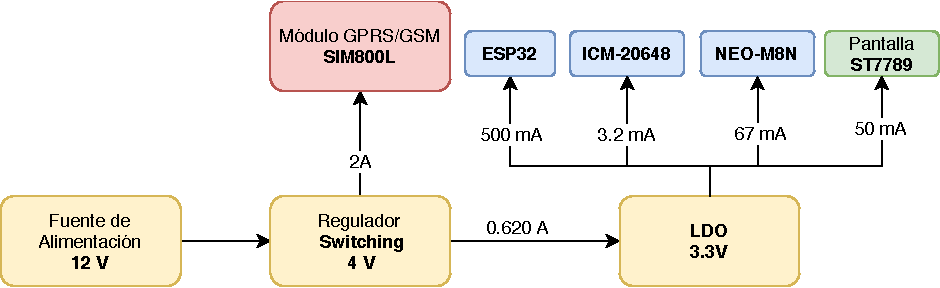
\includegraphics[width=\textwidth]{Bloques_Alimentacion.pdf}
\captionsetup{justification=centering,margin=2cm}
\caption{Diagrama de bloques de las etapas de alimentación con la corriente máxima de cada dispositivo.}
\label{fig:bloques_alim}
\end{figure}

\newpage

Se propone dos etapas de regulación de voltaje debido a que se necesitan 2 niveles de voltaje, \SI{4}{V} y \SI{3.3}{V}. En la primera etapa se usará un regulador switching para obtener \SI{4}{V} de los \SI{12}{V} disponibles en la alimentación. Y en la segunda etapa se usará un LDO (Low Dropout Regulator) para obtener los \SI{3.3}{V} a partir de los \SI{4}{V}. En la Fig.~\ref{fig:bloques_alim} se dispone de manera gráfica e ideal la potencia y las corrientes máximas que deben poder entregar los reguladores de voltaje.



Entonces usando  la Fig.~\ref{fig:bloques_alim} Se tiene que el regulador switching debe poder entregar por lo menos \SI{2.62}{A}. Se selecciona el circuito integrado \textbf{TPS563210} que tiene las características mencionadas en la Tabla~\ref{diag:Switching}

\bgroup
\def\arraystretch{1.5}%  1 is the default, change whatever you need
\begin{table}[htbp!]
\centering
\caption[Características del TPS563210]{Características del TPS563210 \cite{TPS563210}.}
\begin{tabular}{@{}ll@{}}
\toprule
Características & Valor \\ \midrule
Voltaje de entrada & \SI{4.5}{V} - \SI{17}{V} \\
Voltaje de salida & \SI{0.76}{V} - \SI{7}{V} \\
Corriente máxima de operación & \SI{3}{A} \\
Frecuencia de conmutación & \SI{650}{kHz} \\
Temperatura de operación de la juntura & \SI{-40}{\celsius} - \SI{150}{\celsius}\\
Resitencia térmica de juntura-ambiente & \SI{87}{\celsius/W}\\\bottomrule
\end{tabular}
\label{diag:Switching}
\end{table}
\egroup


Se calcula entonces si este regulador switching es capaz de entregar \SI{2.62}{A} o \SI{10.046}{W} sin usar un disipador. Para esto se usa la Ecuación~\ref{eq:disipadores}
\begin{equation}
   T_J=T_A+(R_{\theta JA} \times Potencia_{dis})
   \label{eq:disipadores}
\end{equation}

La $Potencia_{dis}$ en esta ecuación es la potencia disipada la cual se puede calcular a partir de la eficiencia del regulador. Según el datasheet \cite{TPS563210}, se tiene una eficiencia del 93\% cuando el voltaje de salida es \SI{4}{V} y la corriente de salida es \SI{2.6}{A}.
\begin{equation}
    Potencia_{dis}=\frac{Potencia_{salida}}{Eficiencia}\times(1-Eficiencia)
     \label{eq:potencia}
\end{equation}
Usando la Ecuación.~\ref{eq:potencia} se obtiene que el regulador disipará:
 $$Potencia_{dis}=\SI{0.75}{W}$$

Al usar $T_A=\SI{25}{\celsius}$,  $R_{\theta JA}=\SI{87}{\celsius/W}$ y $Potencia_{dis}=\SI{0.75}{W}$ en  la Ecuación~\ref{eq:disipadores} resulta:
$$T_J=\SI{90.25}{\celsius}$$
Esto significa que el regulador podrá operar sin necesidad de usar un disipador para esta aplicación ya que el máximo para $T_J$ es \SI{150}{\celsius}


En la Fig.~\ref{fig:esquem_switching} se puede observar la selección de los componentes externos al TPS563210 usados para obtener una salida de \SI{4}{V} de una fuente de \SI{12}{V}. El primer paso para seleccionar estos componentes fue determinar el voltaje de salida requerido (\SI{4}{V}). En \cite{TPS563210} se tiene que el V\textsubscript{out} seguirá la Ecuación~\ref{eq:vout}.
\begin{figure}[hbtp!]
\centering
\makebox[\textwidth][c]{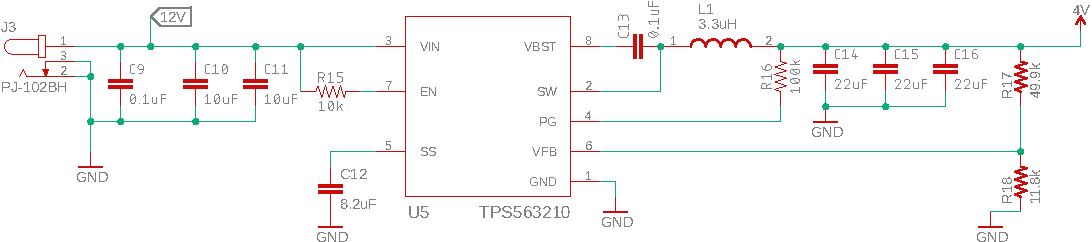
\includegraphics[width=1.2\textwidth]{Switching.pdf}}%
\caption{Esquemático de la implementación del TPS563210.}
\label{fig:esquem_switching}
\end{figure}

\begin{equation}
    V_{out}=0.765\times(1+\frac{R_{17}}{R_{18}})
    \label{eq:vout}
\end{equation}

Para asegurar que $V_{out}=\SI{4}{V}$ se usan resistencias de la serie E96 (con 1\% de tolerancia en su valor). Los valores de $R_{17}$ y $R_{18}$ que cumplen con esta ecuación son $R_{17}=\SI{49.9}{k\ohm}$ y $R_{17}=\SI{11.8}{k\ohm}$.

Luego se recomienda en \cite{TPS563210} usar una inductancia de valor $L_1=\SI{3.3}{\micro H}$ y el IC usa una frecuencia de $f_{SW}=\SI{650}{kHz}$. Además se necesita el valor máximo que el voltaje de entrada V\textsubscript{in} puede tomar, que en este caso será $V_{in}=\SI{16}{V}$ (Esto es debido a fluctuaciones en el voltaje de la batería). Con estos valores se puede determinar los parámetros $Il_{P-P}$, $Il_{PEAK}$,  $I_{LO(RMS)}$ y $I_{CO}$ con las ecuaciones:
\begin{align}
Il_{P-P}&=\frac{V_{out}}{V_{in(MAX)}}\times\frac{V_{in(MAX)}-V_{OUT}}{L_O\times f_{SW}} \label{eq:current1}\\
Il_{PEAK}&=I_{o}+\frac{Il_{P-P}}{2} \label{eq:current2}\\
I_{LO(RMS)}&=\sqrt{I_o^2+\frac{1}{12}Il_{P-P}^2} \label{eq:current3} \\
I_{CO}&=\frac{V_{out}\times (V_{in}-V_{out})}{\sqrt{12}\times V_{in}\times L_{O} \times f_{Sw}} \label{eq:current4}
\end{align}

El resultado de las Ecuaciones \ref{eq:current1}, \ref{eq:current2}, \ref{eq:current3} y \ref{eq:current4} son:
\begin{align*}
Il_{P-P}&=\SI{1.398}{A} &
Il_{PEAK}&=\SI{3.319}{A}&
I_{LO(RMS)}&=\SI{2.79}{A} &
I_{CO(RMS)}&=\SI{0.02}{A}
\end{align*}

Se selecciona entonces el inductor CLF7045NIT-3R3N-D de \SI{3.3}{\micro H} que soporta los parámetros mencionados anteriormente \cite{Inductor} y 3 capacitores C3216X5R0J226M en la salida de \SI{22}{\micro F}  que soporta hasta \SI{4}{A} RMS. Los capacitores de entrada y las demás resistencias se colocan por recomendación de \cite{TPS563210}.

Ahora es momento de elegir el regulador LDO. Para esta etapa se usará el IC \textbf{LT1764A} que posee las características mencionadas en la Tabla~\ref{diag:LDO}.

\bgroup
\def\arraystretch{1.5}%  1 is the default, change whatever you need
\begin{table}[htbp!]
\centering
\caption[Características del LT1764A]{Características del LT1764A \cite{LT1764A}.}
\begin{tabular}{@{}ll@{}}
\toprule
Características & Valor \\ \midrule
Voltaje de entrada & \SI{2.7}{V} - \SI{20}{V} \\
Voltaje de salida & \SI{3.3}{V} \\
Corriente máxima de operación & \SI{3}{A} \\
Dropout Voltage & \SI{340}{mV} a \SI{3}{A} \\
Temperatura de operación de la juntura & \SI{-40}{\celsius} - \SI{150}{\celsius}\\
Resitencia térmica de juntura-ambiente & \SI{30}{\celsius/W}\\\bottomrule
\end{tabular}
\label{diag:LDO}
\end{table}
\egroup

En la Fig.~\ref{fig:LDO} se puede observar la selección de componentes externos y el esquemático propuesto para el LT1764A.

\begin{figure}[hbtp!]
\centering
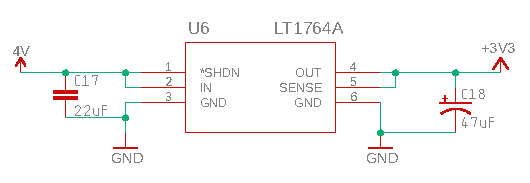
\includegraphics[width=\textwidth]{LDO.pdf}
\caption{Esquemático de la implementación del LT1764A.}
\label{fig:LDO}
\end{figure}

Se comenzará por realizar el análisis térmico de este integrado. La potencia disipada se calcula usando la Ecuación~\ref{eq:pot_LDO}.
\begin{equation}
    Potencia_{dis}=I_{OUT(MAX)}\times(V_{IN(MAX)}-V_{OUT})+I_{GND}\times V_{IN(MAX)} \label{eq:pot_LDO}
\end{equation}
Se reemplazan los siguientes valores en esta ecuación:
\begin{align*}
    V_{OUT}&=\SI{3.3}{V}&
    V_{IN(MAX)}&=\SI{4}{V}&
    I_{OUT(MAX)}&=\SI{0.62}{A}&
    I_{GND}&=\SI{20}{mA}&
\end{align*}
Y se obtiene el siguiente resultado:
$$ Potencia_{dis}=\SI{0.514}{W}$$

Ahora se aplica la Ecuación~\ref{eq:disipadores} con la que obtendremos la Temperatura de la juntura ($T_J$) que se alcanzará al disipar esa potencia.
$$ T_J=\SI{40.42}{\celsius}$$
Como la $T_{J(MAX)}=\SI{150}{\celsius}$, se puede afirmar que no se necesita disipador para usar este regulador. Por otro lado, Los capacitores C\textsubscript{17} y C\textsubscript{18} toman valores recomendados en \cite{LT1764A}. Con el sistema de alimentación definido se puede graficar el diagrama de bloques completo del sistema (Fig.~\ref{fig:Bloques_comp}). En esta ocasión se colocaron los valores promedio de corriente que consumirá cada dispositivo. Observando este diagrama se puede obtener la potencia promedio que consumirá el dispositivo $P_{prom}=\SI{2.66}{W}$.

\begin{figure}[hbtp!]
\centering
\makebox[\textwidth][c]{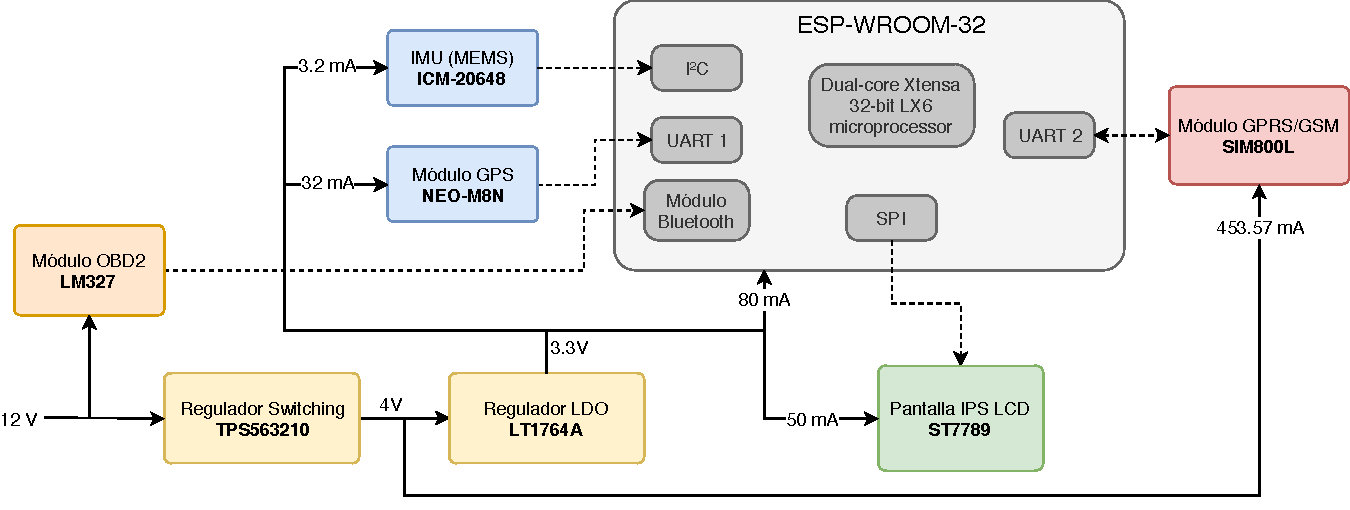
\includegraphics[width=1.2\textwidth]{Bloques_total.pdf}}%
\caption{Diagrama de bloques completo del sistema.}
\label{fig:Bloques_comp}
\end{figure}


\subsection{Diseño del PCB}
A continuación se incluirá el diseño del PCB de doble capa en el que irán todos los componentes antes mencionados.

\begin{figure}[hbtp!]
\centering
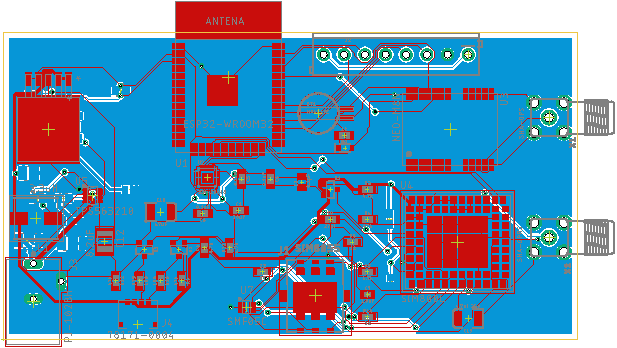
\includegraphics[width=\textwidth]{Board.pdf}
\caption{Diseño del PCB.}
\label{fig:Board}
\end{figure}
